% !TeX root = ../main.tex
\section{Mô hình kinh doanh}

\subsection{Mô hình hoạt động cơ bản của dịch vụ}

Mô hình hoạt động của hệ thống Mutux được thiết kế nhằm đảm bảo sự minh bạch, an toàn và tiện lợi cho cả Người thuê (Renter) và Người cho thuê (Lender), dưới sự giám sát của Quản trị viên (Admin).

\subsubsection{Sơ đồ Use Case (Use Case Diagram)}

Sơ đồ Use Case mô tả các tính năng chính mà các tác nhân (Actor) có thể tương tác với hệ thống. Hệ thống Mutux có 3 tác nhân chính:

\begin{itemize}
    \item \textbf{Người thuê (Renter):} Tìm kiếm, đặt thuê thiết bị, thanh toán và đánh giá.
    \item \textbf{Người cho thuê (Lender):} Đăng tải thiết bị, quản lý yêu cầu thuê, giao dịch và quản lý doanh thu.
    \item \textbf{Quản trị viên (Admin):} Phê duyệt KYC, duyệt thiết bị, giải quyết tranh chấp (Dispute resolution) và quản lý hệ thống.
\end{itemize}

\begin{figure}[H]
    \centering
    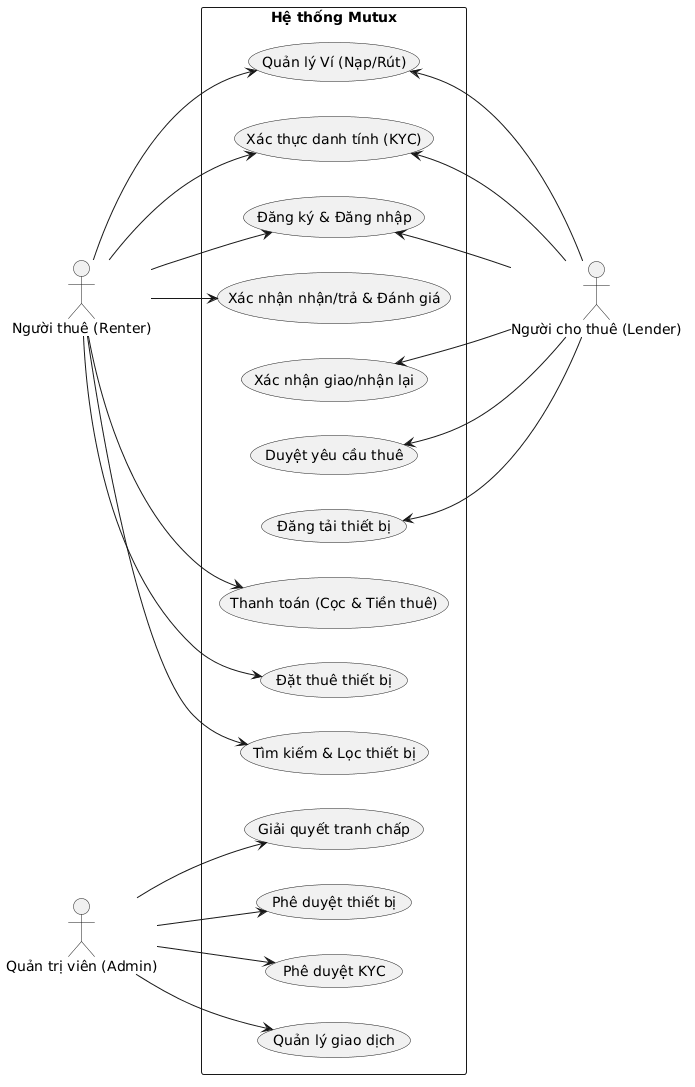
\includegraphics[width=0.95\textwidth]{../PA2/img/usecase.png}
    \caption{Sơ đồ Use Case của hệ thống Mutux}
    \label{fig:usecase}
\end{figure}

\subsubsection{Sơ đồ Hoạt động (Activity Diagram)}

Quy trình cốt lõi nhất của Mutux là luồng Đặt thuê và Bàn giao thiết bị. Hệ thống áp dụng cơ chế thanh toán tạm giữ (Escrow) và quy trình xác thực minh chứng (Proof) để bảo vệ cả hai bên.

Quy trình cơ bản diễn ra theo các bước sau:
\begin{enumerate}
    \item \textbf{Đặt thuê:} Người thuê tìm kiếm thiết bị, chọn ngày thuê và gửi yêu cầu.
    \item \textbf{Phê duyệt:} Người cho thuê xem xét và chấp nhận yêu cầu.
    \item \textbf{Thanh toán:} Người thuê tiến hành thanh toán tiền thuê và tiền cọc. Số tiền này được chuyển vào ví hệ thống (Escrow) chờ xử lý.
    \item \textbf{Giao nhận:} Người cho thuê bàn giao thiết bị và cập nhật hình ảnh minh chứng (Proof). Người thuê nhận, kiểm tra và xác nhận trên hệ thống.
    \item \textbf{Hoàn trả:} Khi hết hạn, người thuê trả lại thiết bị kèm hình ảnh minh chứng. Người cho thuê nhận và xác nhận tình trạng.
    \item \textbf{Quyết toán:} Hệ thống hoàn lại tiền cọc cho người thuê và chuyển tiền thuê (sau khi trừ phí nền tảng) vào ví của người cho thuê. Nếu có vấn đề phát sinh, Admin sẽ can thiệp để giải quyết tranh chấp.
\end{enumerate}

\begin{figure}[H]
    \centering
    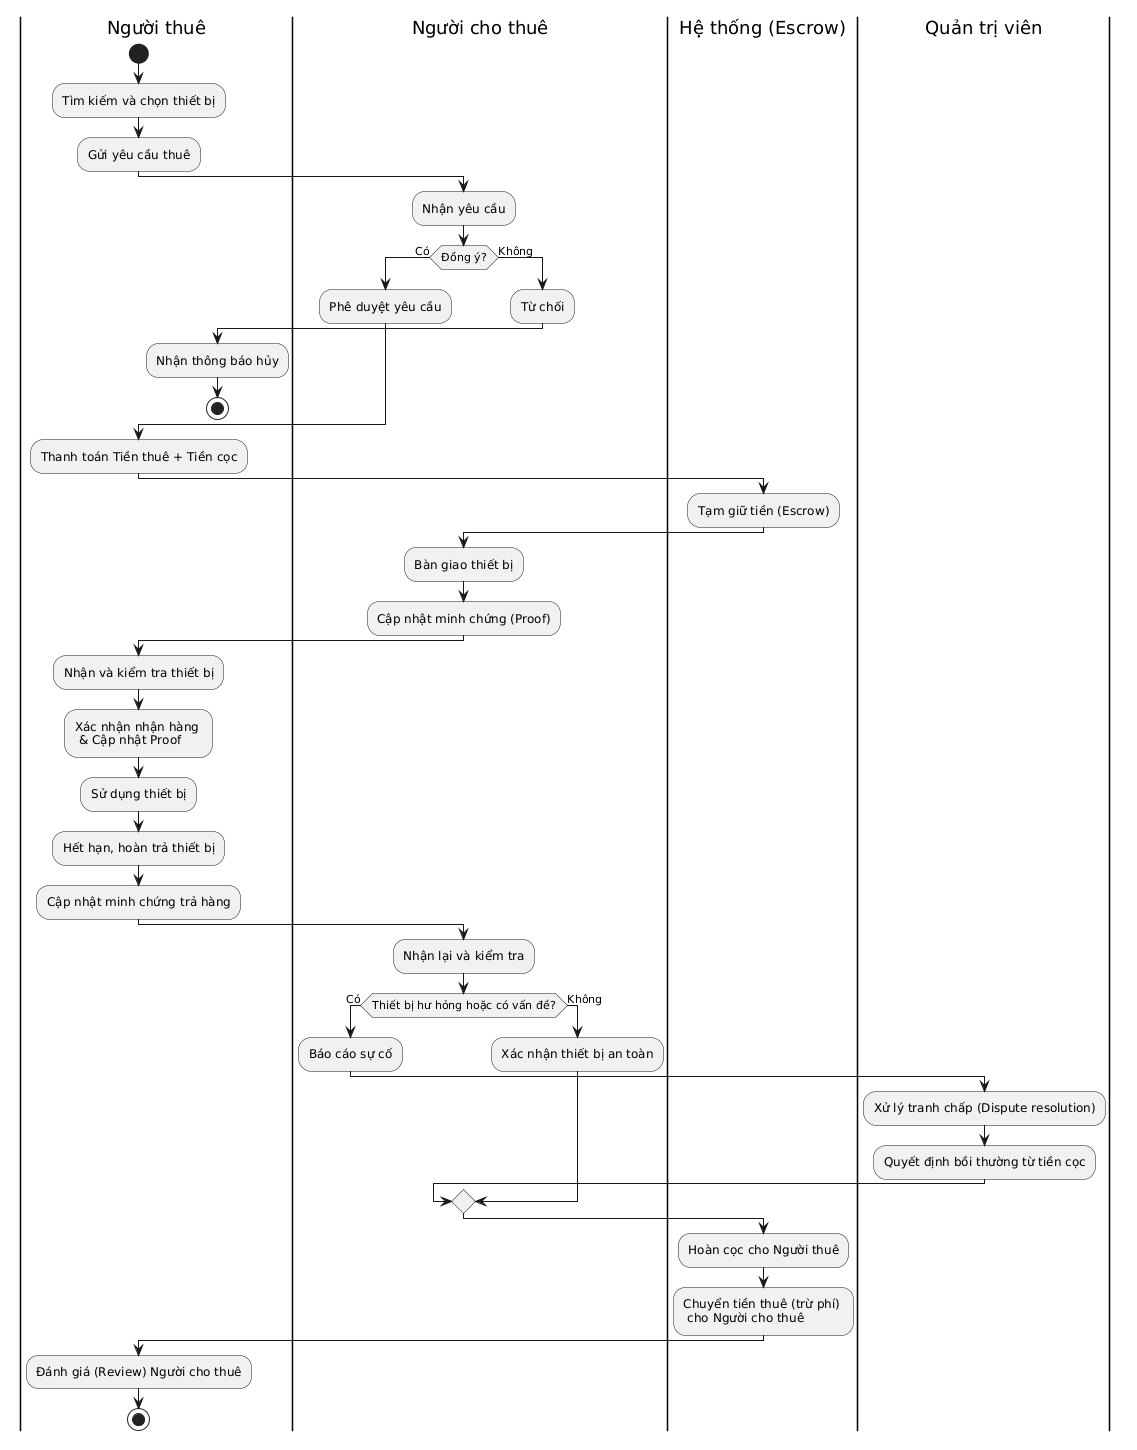
\includegraphics[width=0.9\textwidth]{../PA2/img/activity.png}
    \caption{Sơ đồ Hoạt động quy trình thuê thiết bị trên Mutux}
    \label{fig:activity}
\end{figure}

\subsection{Mô hình doanh thu của dự án}
Mutux vận hành theo mô hình trung gian kết nối (Marketplace) kết hợp dịch vụ bảo vệ thanh toán (Escrow). Thay vì phụ thuộc hoàn toàn vào phí thuê thiết bị – phần doanh thu vốn dĩ thuộc về đối tác cho thuê – Mutux đa dạng hóa nguồn doanh thu thông qua các giao dịch B2C, các dịch vụ dành cho đối tác B2B và các chương trình hợp tác với đối tác thanh toán. Mô hình này giúp tối ưu hóa biên lợi nhuận thông qua việc khai thác luồng giao dịch từ cả hai phía cung và cầu.


\subsection{Các nguồn doanh thu dự kiến}

\textbf{Nguồn doanh thu cơ sở (từ Giao dịch B2C):}
\begin{itemize}
    \item \textbf{Phí nền tảng (Take Rate):} Đây là nguồn thu chủ lực của Mutux. Hệ thống sẽ tự động trích xuất hoa hồng \textbf{30\%} trên tổng giá trị tiền thuê của mỗi giao dịch thành công.
\end{itemize}

\textbf{Nguồn doanh thu Dịch vụ (Theo lộ trình 2 giai đoạn):}
\begin{itemize}
    \item \textbf{Dịch vụ Hỗ trợ tiền cọc (Deposit Advance Service):} Trong giai đoạn đầu, Mutux triển khai cơ chế hỗ trợ ứng trước tiền cọc cho một số khách hàng đáp ứng điều kiện xác minh danh tính (eKYC) và tiêu chí đánh giá nội bộ. Nền tảng thu \textbf{phí dịch vụ là 30.000 VNĐ} cho mỗi tháng người dùng sử dụng tiền cọc để nạp vào ví. Dịch vụ này sử dụng mô hình hợp tác với các đối tác tài chính (BNPL như MoMo, Fundiin) để giảm áp lực vốn lưu động và mở rộng khả năng phục vụ. Mutux không trực tiếp cung cấp dịch vụ tín dụng. Trong giai đoạn đầu, nền tảng chỉ đóng vai trò kết nối người dùng với đối tác BNPL hoặc các tổ chức tài chính. Mutux thu hoa hồng giới thiệu hoặc phí dịch vụ từ đối tác. Đối với rủi ro hỏng hóc/mất mát thiết bị, Mutux áp dụng cơ chế Giữ tiền Escrow + Định danh eKYC + Trừ trực tiếp tiền cọc/ví đối soát nếu xảy ra tranh chấp.
\end{itemize}

\textbf{Nguồn doanh thu mở rộng (từ Đối tác B2B - Triển khai sau 1 năm):}
\begin{itemize}
    \item \textbf{Phí quảng cáo và Đẩy tin (Featured Listings):} Nhằm tối ưu hóa khả năng bán hàng cho các shop gaming gear, Mutux thu phí để hiển thị ưu tiên sản phẩm của họ trên trang chủ hoặc khi người dùng tìm kiếm. 
    \item \textbf{Hoa hồng bán chéo (Cross-selling):} Đóng vai trò như một kênh "Dùng thử trước khi mua", Mutux sẽ nhận hoa hồng môi giới khi người thuê quyết định "mua đứt" thiết bị sau quá trình trải nghiệm.
\end{itemize}


% !TeX root = ../main.tex
\subsection{Các nhóm chi phí chính}
Để vận hành và phát triển nền tảng, cơ cấu chi phí của Mutux được phân bổ cho 12 tháng đầu tiên như sau:

\begin{table}[htbp]
    \centering
    \caption{Phân bổ chi phí dự kiến năm 1}
    \resizebox{\textwidth}{!}{%
    \begin{tabular}{@{}lrl@{}}
        \toprule
        \textbf{Hạng mục chi phí} & \textbf{Mức dự kiến (VNĐ)} & \textbf{Phân bổ} \\
        \midrule
        \textbf{Marketing (CAC, Khuyến mãi)} & 120.000.000 & Ads mạng xã hội, voucher giải quyết Cold-start. \\
        \textbf{Phát triển Sản phẩm (Tech/R\&D)} & 30.000.000 & Phát triển tính năng Escrow, tích hợp eKYC, PayOS. \\
        \textbf{Hạ tầng Công nghệ (Server, API)} & 100.000.000 & Phí Cloud Server, OTP, API đối soát, Domain name,... \\
        \textbf{Vận hành \& Nhân sự (Operations)} & 180.000.000 & Đội ngũ thiết kế, tạo sản phẩm, đội ngũ CSKH và giải quyết tranh chấp. \\
        \textbf{Tư vấn Pháp lý} & 30.000.000 & Soạn thảo hợp đồng điện tử, quy định bảo mật. \\
        \textbf{Quỹ Dự phòng} & 20.000.000 & Dự phòng rủi ro tài sản và thanh khoản. \\
        \midrule
        \textbf{TỔNG CHI PHÍ DỰ KIẾN (NĂM 1)} & \textbf{480.000.000} & \\
        \bottomrule
    \end{tabular}%
    }
\end{table}

\subsection{Phân tích mô hình phí và vận hành}

\subsubsection{Cách hoạt động và các khoản phí}

Mutux hoạt động theo mô hình marketplace kết nối ba bên chính: người thuê gear, shop hoặc chủ gear, và nền tảng Mutux. Trong phiên bản mở rộng, Mutux có thể kết nối thêm đối tác tài chính để triển khai dịch vụ Cọc Trả Sau, tức hỗ trợ vay hoặc bảo chứng phần cọc theo giá trị sản phẩm.

Các khoản phí chính trong mô hình gồm:

\begin{itemize}
    \item \textbf{Phí thuê gear}: người thuê trả theo ngày hoặc theo gói ngắn hạn. Ví dụ, một tay cầm trị giá khoảng 2.000.000 đồng có thể được cho thuê với giá 10.000 đồng/ngày; nếu thuê ba ngày thì phí thuê là 30.000 đồng.
    \item \textbf{Hoa hồng nền tảng}: Mutux lấy khoảng 10\%--20\% trên phí thuê thành công. Nếu phí thuê là 30.000 đồng, nền tảng có thể nhận 3.000--6.000 đồng, phần còn lại thuộc về shop hoặc chủ gear.
    \item \textbf{Tiền cọc truyền thống}: người thuê đặt cọc để bảo vệ tài sản cho bên cho thuê. Với thiết bị trị giá khoảng 1.800.000--2.000.000 đồng, tiền cọc có thể bằng toàn bộ giá trị sản phẩm. Khoản này không phải doanh thu của Mutux mà là khoản đảm bảo, được hoàn lại khi người thuê trả thiết bị đúng tình trạng.
    \item \textbf{Phí Cọc Trả Sau hoặc phí vay cọc}: nếu người dùng không muốn hoặc không đủ khả năng ứng trước toàn bộ tiền cọc, họ có thể chọn dịch vụ hỗ trợ cọc. Ví dụ, thay vì khóa trước 2.000.000 đồng tiền cọc cho một món gear, người dùng trả thêm khoảng 5.000--10.000 đồng phí vay/bảo chứng cọc cho một đơn thuê ngắn ngày. Mức phí này được thiết kế rất thấp, tương tự các nền tảng ví trả sau hoặc SPayLater, còn tiền thuê/mượn thiết bị vẫn do người cho thuê đặt ra.
    \item \textbf{Hoa hồng từ đối tác tài chính}: nếu dịch vụ Cọc Trả Sau được triển khai qua ngân hàng, ví điện tử hoặc công ty tài chính được cấp phép, Mutux có thể nhận phần chia sẻ doanh thu hoặc hoa hồng giới thiệu từ giao dịch này.
    \item \textbf{Hoa hồng mua sau thuê}: nếu người dùng thuê thử và quyết định mua sản phẩm từ shop, Mutux có thể nhận hoa hồng từ giao dịch mua. Shop cũng có thể trừ một phần phí thuê vào giá bán để tăng tỷ lệ chuyển đổi.
    \item \textbf{Gói thành viên}: người dùng trả phí định kỳ để được giảm phí thuê, giảm phí bảo lãnh cọc, ưu tiên thuê gear hot hoặc nhận ưu đãi giao nhận.
    \item \textbf{Gói dịch vụ cho shop}: shop có thể trả phí để đăng nhiều thiết bị hơn, dùng dashboard quản lý đơn thuê, được quảng bá sản phẩm hoặc tiếp cận nhóm khách có nhu cầu mua sau khi dùng thử.
\end{itemize}

Với cách vận hành này, doanh thu của Mutux không phụ thuộc hoàn toàn vào phí thuê gear. Phần phí thuê chủ yếu cần đủ hấp dẫn để shop và chủ gear có động lực đưa thiết bị lên nền tảng. Lớp doanh thu quan trọng hơn nằm ở hoa hồng, phí vay/hỗ trợ cọc, chia sẻ doanh thu với đối tác tài chính và giao dịch mua sau thuê.

\subsubsection{So sánh hai cách đặt cọc}

Điểm khác biệt quan trọng của Mutux là cho người dùng lựa chọn giữa đặt cọc truyền thống và Cọc Trả Sau. Ví dụ, người dùng thuê một tay cầm trị giá 2.000.000 đồng trong ba ngày, với phí thuê 10.000 đồng/ngày.

\begin{center}
\begin{tabular}{>{\raggedright\arraybackslash}p{0.36\textwidth} >{\raggedleft\arraybackslash}p{0.22\textwidth} >{\raggedleft\arraybackslash}p{0.24\textwidth}}
\toprule
\textbf{Khoản mục} & \textbf{Cọc truyền thống} & \textbf{Cọc Trả Sau} \\
\midrule
Giá trị tay cầm & 2.000.000đ & 2.000.000đ \\
Phí thuê 3 ngày & 30.000đ & 30.000đ \\
Tiền cọc ứng trước & 2.000.000đ & 0đ \\
Phí vay/hỗ trợ cọc & 0đ & 5.000--10.000đ \\
Tổng tiền ban đầu & 2.030.000đ & 35.000--40.000đ \\
\bottomrule
\end{tabular}
\end{center}

Như vậy, với cùng một món tay cầm trị giá 2.000.000 đồng, cách thuê truyền thống khiến người dùng phải chuẩn bị 2.030.000 đồng ngay từ đầu, còn Cọc Trả Sau chỉ cần khoảng 35.000--40.000 đồng cho ba ngày thuê. Khoản chênh lệch này làm mô hình đủ tiện và hợp lý hơn cho sinh viên, người mới chơi eSports hoặc người có ngân sách hạn chế: họ vẫn được dùng thử thiết bị thật, bên cho thuê vẫn có cơ chế bảo vệ tài sản nếu hư hỏng hoặc mất đồ, còn Mutux có thêm nguồn thu ngoài hoa hồng thuê.

\subsubsection{Tính khả thi về vận hành}

Ở giai đoạn MVP, Mutux chưa cần tự đứng ra cho vay hoặc triển khai sản phẩm tài chính thật. Hướng an toàn hơn là mô phỏng flow Cọc Trả Sau để chứng minh nhu cầu, sau đó mới hợp tác với ngân hàng, ví điện tử hoặc công ty tài chính được cấp phép nếu muốn triển khai thật.

Để mô hình vận hành được, nền tảng cần có các cơ chế cơ bản:

\begin{itemize}
    \item Xác minh danh tính người thuê trước khi cho thuê thiết bị có giá trị cao.
    \item Kiểm tra và ghi nhận tình trạng thiết bị trước và sau khi thuê.
    \item Quy định rõ phí trả muộn, phí hư hỏng, mất thiết bị và điều kiện hoàn cọc.
    \item Theo dõi trạng thái thiết bị: available, booked, renting, returned, maintenance.
    \item Giới hạn giá trị hỗ trợ cọc theo độ tin cậy của người thuê.
    \item Ưu tiên thử nghiệm với một số shop hoặc cộng đồng gamer nhỏ trước khi mở rộng.
\end{itemize}

Nhờ đó, Mutux có thể kiểm chứng nhu cầu thị trường trước, đồng thời tránh rủi ro pháp lý khi chưa đủ điều kiện tự cung cấp dịch vụ tài chính.
